\documentclass[letterpaper,10pt]{article}

\usepackage{titling}
\usepackage{listings}
\usepackage{url}
\usepackage{setspace}
\usepackage{subfig}
\usepackage{sectsty}
\usepackage{pdfpages}
\usepackage{colortbl}
\usepackage{multirow}
\usepackage{multicol}
\usepackage{relsize}
\usepackage{amsmath}
\usepackage{fancyvrb}
\usepackage{amsmath,amssymb,amsthm,graphicx,xspace}
\usepackage[titlenotnumbered,noend,noline]{algorithm2e}
\usepackage[compact]{titlesec}
\usepackage{XCharter}
\usepackage[T1]{fontenc}
\usepackage{tikz}
\usetikzlibrary{arrows,automata,shapes,trees,matrix,chains,scopes,positioning,calc}
\tikzstyle{block} = [rectangle, draw, fill=blue!20, 
    text width=2.5em, text centered, rounded corners, minimum height=2em]
\tikzstyle{bw} = [rectangle, draw, fill=blue!20, 
    text width=4em, text centered, rounded corners, minimum height=2em]

\newcommand{\CPP}{C\nolinebreak\hspace{-.05em}\raisebox{.4ex}{\tiny\bf +}\nolinebreak\hspace{-.10em}\raisebox{.4ex}{\tiny\bf +}}
\def\CPP{{C\nolinebreak[4]\hspace{-.05em}\raisebox{.4ex}{\tiny\bf ++}}}

\let\LaTeXtitle\title
\renewcommand{\title}[1]{\LaTeXtitle{\textsf{#1}}}


\addtolength{\oddsidemargin}{-1.000in}
\addtolength{\evensidemargin}{-0.500in}
\addtolength{\textwidth}{2.0in}
\addtolength{\topmargin}{-1.000in}
\addtolength{\textheight}{1.75in}
\addtolength{\parskip}{\baselineskip}
\setlength{\parindent}{0in}
\renewcommand{\baselinestretch}{1.5}

\singlespace

\begin{document}

\lecture{25 --- Profiling: Observing Operations}{\term}{Jeff Zarnett}

\section*{Observations Precede Conclusions}

Think back to the beginning of the course when we did a quiz on what operations are fast and what operations are not. The important takeaway was not that we needed to focus on how to micro-optimize this abstraction or that hash function, but that our intuition about what is fast and what is slow is often wrong. Not just at a macro level, but at a micro level. You may be able to narrow down that this computation of $x$ is slow, but if you examine it carefully\ldots what parts of it are slow?

If you don't use tools, then you end up guessing. You just make some assumptions about what you think is likely to be slow and try to change it. You've probably heard the famous quotation before, but here it is in its full form:

\begin{quote}
\textit{Programmers waste enormous amounts of time thinking about, or worrying about, the speed of noncritical parts of their programs, and these attempts at efficiency actually have a strong negative impact when debugging and maintenance are considered. We should forget about small efficiencies, say about 97\% of the time: premature optimization is the root of all evil. Yet we should not pass up our opportunities in that critical 3\%.}
\end{quote}
	\hfill -- Donald Knuth

So going about this blindly is probably a waste of time. You might be fortunate and optimize a slow part, but we should really follow one of my favourite rules: ``don't guess, measure!'' So, to make your programs or systems fast, you need to find out what is currently slow and improve it (duh!). Up until now in the course it's mostly been about ``let's speed this up'', but we did not take much time to decide what we should speed up (though you maybe did this on an assignment\ldots?).

The general idea is, collect some data on what parts of the code are taking up the majority of the time. This can be broken down into looking at what functions get called, or how long functions take, or what's using memory\ldots

\paragraph{Why Observation?} We're talking here about the idea of observation of our program, which is a little bit more inclusive than just measuring things, because we may observe things that are hard or impossible to quantify. Observing the behaviour of the program will obviously be super helpful in terms of figuring out what -- if anything -- to change. We have several different ways of looking at the situation, including logs, counters, profiling, and traces. Differences between them, briefly~\cite{usd}:

\begin{itemize}
	\item \textbf{Counters} are, well, a stored count of the occurrences of something: how many times we had a cache miss, how many times we called \texttt{foo()}, how many times a user logged in...
	\item \textbf{Profiles} are higher-level overviews of what the program is doing, where time is going in aggregate, and how long certain operations take.
	\item \textbf{Traces} are recordings that show the sequence of events that the program is doing, so we can understand the runtime behaviour and how we got to the state we are in.
\end{itemize}

We'll return to profilers later, because it's a big topic, but for now we'll start with traces and counters.

\subsection*{Tracing: Logging}
We'll start with the idea of logging. It's an effective way of finding out what's going on in your program as it executes, and probably all of us have use print statements as a form of debugging, but also as a form of tracing. When we're running a small program, we don't always make the log messages very nice, but in a production system, logs typically have a timestamp, a message, and some attributes. The timestamp is helpful for organizing and searching the logs. 

In~\cite{usd} it's recommended that if there can be only one tool for observing your program's execution, it is logging. This is because logging can tell you things about how much work the software did in a time period, when things are busy, which transactions are slow, when the service is down, etc. This probably matches well with our intuition that printf debugging or tracing is a good first option to figure out what's going on.

Given that we want to log, we do have to consider how often to log, and what should be in the content of it. If we don't log the information, there may not be any good way to recover that information again. But we could also drown out useful information if we log too many (irrelevant) things. Logs typically have levels, like error, warning, info, debug... These can make it easier to spot just the information that is relevant.

A typical approach is to log an incoming request (input) and the outgoing response (output), and maybe some steps in between. We want to link the different things together (perhaps with attributes) so that we can see what happened. Here's a made-up example that doesn't show the time stamps or attributes:

\begin{verbatim}
Received request: update plan of company 12345 to ULTIMATE
Retrieving company 12345
Verifying eligibility for upgrade of company 12345 from BASIC to ULTIMATE
Company 12345 is not eligible for upgrade due to: unpaid invoices > 0
Returning response: update of company 12345 to ULTIMATE is DECLINED
\end{verbatim}

We can see the various steps of the process and quickly understand what happened, because the logs show us the request, the stages of handling the request, and the response. In this example I intentionally added a decision and logged the reason for the decision. That's preferable to making someone guess why the answer was no when looking at the logs.

Choosing the timestamps strategy is also interesting; the level of precision you need in the logging depends on the timescales of your execution. When running processes that take tens of seconds, you could probably be satisfied with down to the thousandth of a second; if things run super fast then we might need microsecond or nanosecond resolution~\cite{usd}. Time zones also matter, but I'm going to recommend using UTC because it doesn't have weird things like Daylight Savings Time where you can get a jump in the time forward or back. And back is worse because it means a certain minute appears to happen more than once (defeating our normal expectation of linear time). It also avoids issues where the California team thinks it's Monday and the Singapore team thinks it's Tuesday. UTC might be weird, though, if your application is running on a Mars Rover; at that point you might as well use Stardates (Captain's Log, Stardate 46119.1...).

As I already said, logging every request might be too noisy to actually find anything in the resulting data. The ability to search and sort helps, but it can still be going by too fast to realistically assess in real-time. Log aggregation services exist and they can help, especially when trying to do a retrospective.

Typically, adding any relevant attributes is very helpful to identify what has happened or to correlate knowledge. If we can see in the attributes that updates for plans of companies always take ten times longer if the company's address is in Portugal, that's actually a useful observation. We can take that information and put it in the bug ticket and ideally help the developer -- even if it's our future selves -- to find the issue and resolve it.

With that said: there's such a thing as too much detail in logging. Logs should always redact personally-identifiable information such as people's names, contact information, medical records, etc. Unless the logs are really kept in secure storage with appropriate access controls, they can be seen by people who shouldn't have that information. Why should, for example, a developer on the website team have access to the banking details of a customer? My opinion: they shouldn't. And it's not just my opinion, but also the opinion of people like the Privacy Commissioner of Canada, whom you probably do not want to anger.

One way that we get into the situation of over-logging is if it's difficult or impossible to use other tools on the program or to have (read-)access to the database. If someone is trying to debug the behaviour of the program it might seem sensible to log just about everything because it's frustrating to try to debug a problem with incomplete information. 

So we are aiming for a balance: include the relevant information that would let us spot patterns or correlate with other data sources, but not so much that the important information is lost or that PII is exposed.

There is a third way that a program logging too much, beyond drowning out key info or logging PII, and that's if the overhead of tracing is significant. Normally we're happy to accept some small slowdown in our program to have traceability, but let's try to put some numbers to tracing overhead. 

Some quick, off-the-cuff figures from~\cite{usd}:
\begin{itemize}
	\item If we ask the CPU trace tool to track every conditional branch taken, that would be about a $20\times$ slowdown. This amount of overhead would be acceptable if we're debugging the program on a development machine (own laptop or testing deployment), but certainly not in a production environment.
	\item If we ask for a timestamp at every function call and return in our program the slowdown is around $1.2-1.5\times$. This may (emphasis on may) be acceptable in a production environment if the task is not time-critical, but only temporarily while experimenting or observing.
	\item If we ask for a timestamp of every system call entry and exit (user-space to kernel transition and back), that might be much less than $1\%$ overhead. This would likely be acceptable in a production environment for all but the most time-critical of operations and could remain in place at all times.
\end{itemize}

That covers tracing the CPU. What about memory? If you've used Valgrind\footnote{So, we used to cover Valgrind in this course. That made sense when it was C and \CPP~but we used to discuss it in Rust too. While the Helgrind part might help you find lock acquisition issues, for the most part students found that there were too many false positives around memcheck and it was just causing students to stress about losing marks. So... away with it.} before, you know it. If you haven't, as I say to the ECE~252 students: The target program then runs under the ``supervision'' of the tool. This results in running dramatically slower than normal, but you get additional checks and monitoring of the program. Why? Valgrind checks every memory read and write for validity (is the variable initialized? Is it off the end of an array? All those fun things that we, fortunately, no longer think about in Rust), but also records information about where memory is allocated to help the programmer in tracking down the genesis of a memory leak. When execution of the program ends, Valgrind shows the stack trace of the path that led to the allocation that was leaked. That's pretty neat!

A disk trace tool would most likely have extremely tiny overhead because the speed of the disk as compared to the CPU is very slow. Something similar goes for the network; the latency is high and speed of the network are slow compared to what the CPU can do~\cite{usd}. 

Tracing also can play a role in identifying deadlocks and delays in threads caused by waiting for locks: simply log every lock and unlock. But we might really be only interested in the locks where there is contention, i.e., threads are sometimes or often failing to acquire the lock because it's held by another thread~\cite{usd}. After all, if our intention is to observe the behaviour of the program with the intention of improving performance, the part where a thread isn't getting what it wants immediately and must wait is much more interesting than the part where everything is fine and there are no delays.

\paragraph{Space, the Final Frontier.} Whatever trace strategy we choose, the trace itself takes up space. If we are producing a very large amount of data, it won't all fit in memory and has to go on disk. It's possible that the amount of data that we produce will fill up the disk very quickly, or arrive so fast that the disk cannot keep up. In~\cite{usd} there's a quick calculation that says a main memory system with 20 GB/s bandwidth and 64-byte cache lines that records up to 8 bytes of data per trace entry could result in producing data at a rate of 2.4 GB per second! That's a rather overwhelming amount of data -- even if you could write it all out to disk fast enough, it would fill up an 8 TB hard drive in just under an hour. Either we need to capture less data by recording fewer things or by recording for a shorter time. Just add this to the reasons why we need to be judicious about how much trace data to capture.

\subsection*{Aggregate Measures (Counters)}
Many profiling tools rely heavily on counters. Counters, as the name suggests, keep a count of events: interrupts, cache misses, data bytes written, calls to function \texttt{do\_magic()}. Keeping track of these numbers is relatively inexpensive (specially when compared to other approaches so counting every occurrence of an event is actually plausible. Counters are a form of aggregation, because we're summing the number of occurrences and at the end of the program we have a total number. The counter any any data derived from it certainly takes much less space than a trace.

The sum is the simplest kind, but other aggregate measures are exactly what they sound like: summaries of data. Calculating the average response time of a request is an aggregate measure: we've summed up the total time per request and divided it by the number of requests in the given period and hopefully the resulting value is a useful one. Asking the computer to calculate the summary is sensible, of course, because it's not realistic to ask a human to look at 50~000 requests and calculate their average time. Some obvious aggregate measures are things like: number of requests, requests broken down by type, average time to respond to a request, percentage of error responses...  

Whatever aggregate measures we use, they are useful only with context.  Suppose that after my pull request is merged, the average login time for a user is 0.75 seconds; is that a problem? Without a baseline to compare against, I'm not sure. If before my PR it was 0.5 seconds, I made performance much worse and that doesn't sound good; should I revert it and re-work it? Maybe, unless I am intentionally making login slower to make a brute-force password attack more expensive for an attacker. Context is key: the summary tells you some data, but not the reasons.

Another example: if I tell you that a request takes, on average, 1.27 seconds to get a response, is that good or bad? There's, again, no way to say anything about it without a point of reference. Are we being asked to approve or deny a transaction and there's a time limit of 1 second to give our answer (or else a default answer is assumed)? We're missing the target and that's a problem. If instead I said the time limit is 10 seconds, then we have plenty of room. Or do we?

Average time isn't quite enough to know if we're doing well when it comes to time limits. If the average time is 1.27 seconds it does not preclude the possibility that the maximum time is outside the 10 second time limit and that means for some percentage of requests, possibly a large percentage, we're not making the deadline. How hard of a deadline are we talking about? To address this we can look at maximum and 95th percentile kind of aggregate measures as well.

The other way that averages can be misleading is that they misrepresent the bursty nature of the data. If your service receives, on average, 7 requests per second, does that mean it looks like the first, second, or third row below (all from~\cite{usd})?

\begin{center}
	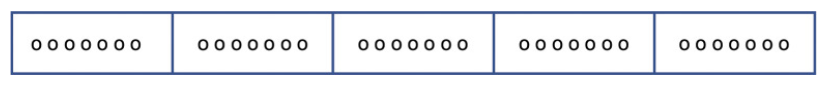
\includegraphics{images/burst1}\\
	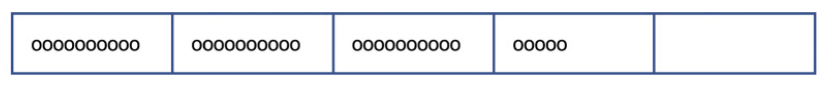
\includegraphics{images/burst2}\\
	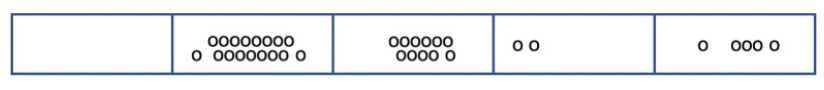
\includegraphics{images/burst3}\\
\end{center}

While the first scenario is really nice and very predictable, is that realistic? Later on in the course we'll talk more about queueing theory and we'll learn that random arrivals and what it means for things to arrive.

When we choose to aggregate our data in some way, we must make a decision about the period of time in question. If our program is going to, say encode a video, the period of time is probably the whole execution time of the task: it took 3h 21 minutes to encode the video and that results in a processing rate of 210.9 frames per second. For services that run indefinitely or when we're impatient, we might want to look at a shorter period of time and consider that. But if we choose the wrong period we'll miss important things: if we look at purchases per hour, if we look at Sunday night that might be misleading as compared to Monday at noon.

\paragraph{Look at the pretty pictures.} 
Often, we want to not just see the raw data, but also the trend in the data; choosing the right visualization is really helpful. Digital speedometers in cars are more accurate than a sweep one in terms of showing you the speed of your vehicle, but the sweeping analog speedometer makes it easier for a person to understand the acceleration (rate of change of that speed). Representing changes in data over time in a graph makes it easier to identify trends or alarming things, and as a bonus, managers and non-technical people love them and love to rely on them. 

Consider just a simple example of the CPU usage graph from my laptop when I compile and run the nbody-parallel code; the blue represents user-space execution and red represents kernel execution:

\begin{center}
	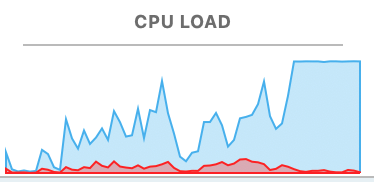
\includegraphics[width=0.3\textwidth]{images/cpu-load.png}
\end{center}

It is obvious in this picture at what point the simulation starts running for real. If we see this and we can identify an operation that starts around the time the CPU is maxed out, we have found something useful.

\paragraph{Dashboards.} If we put together enough pretty pictures, we get a... dashboard! Dashboards are (ideally) more than just pretty pictures of LINE GOES UP. It is instead intended to be a collection of useful graphs (time trends, histograms, etc) that present an easily-digestible summary of the situation. Good dashboards make it clear what's happening and what things need attention. Of course, dashboards tend to make more sense when we have many things to measure; not so much if we're just trying to optimize one specific thing.

\subsection*{Drill-down}
All of this introduction to profiling has really been focused around the higher level ideas for identifying what's happening and what operations, if any, are slow (or slower than expected). Once we know that, for example, importing CSV files with tax rates is slow, we can start to use some profiling tools to identify what is slow inside that functionality.  In the next topic, we'll start by looking at some specific profiling tools and their approaches.



\bibliographystyle{alphaurl}
\bibliography{459}


\end{document}
